\documentclass[aspectratio=169, xcolor=table]{beamer}
\usetheme{Frankfurt} % Theme choice (can be changed)
\usecolortheme{dolphin}
\usepackage{amsmath, amssymb, graphicx, booktabs, multirow}
\usepackage{tikz}
\usetikzlibrary{arrows, positioning, arrows.meta, shapes.geometric,calc}
\usepackage[dvipsnames]{xcolor}
\usepackage{graphicx} % useful if you later want to add icons/images
% ---------------
\usepackage[utf8]{inputenc}
\usepackage[T1]{fontenc}
\usepackage{lmodern}
\usepackage{textcomp}
% ---------------

\title{The Bank of Amsterdam and the Limit of Fiat Money \\ \small Bolt, Wilko; Frost, Jon; Shin, Hyun Song; Wierts, Peter \\ \small Journal of Political Economy, 2024}
\author{Lorenzo Gorini \newline Vivien Bonten \newline Yiwen Jin }
\institute{Bocconi University}
\date{October 15, 2025}


\begin{document}

\AtBeginSection[]{
  \begin{frame}{Presentation Outline}
    \footnotesize
    \tableofcontents[
      currentsection,
      subsectionstyle=show/show/hide, % show subsections of current section only
      sectionstyle=show/shaded        % highlight current section
    ]
  \end{frame}
}

%------------------------------------------------
\begin{frame}
  \titlepage
\end{frame}
%------------------------------------------------

% Outline Slide
\begin{frame}{Presentation Outline}
  \tableofcontents
\end{frame}

%------------------------------------------------
% Section 1: Introduction
\section{Introduction}

\begin{frame}{Historical Context (1/2)}


  \begin{columns}
    \begin{column}{0.55\textwidth}
      \begin{itemize}
        \item Early 17th-century Europe: pervasive \textbf{coin debasement} $\Rightarrow$ severe \textbf{valuation frictions} in trade.
        \item Amsterdam as a major \textbf{international trading hub}: high settlement volumes required \textbf{reliable unit of account} and efficient \textbf{large-value payments}.
        \item Emergence of \textbf{fiat money to overcome heterogeneous coin quality}; \textbf{AGIO} (premium/discount) measures bank money’s quality vs. coin.
      \end{itemize}
    \end{column}
    \begin{column}{0.4\textwidth}
      \begin{center}
        \includegraphics[width=0.87\linewidth]{pasted-images/amsterdam.png}
      \end{center}
    \end{column}
  \end{columns}
\end{frame}

\begin{frame}{Historical Context (2/2)}
  \begin{itemize}
    \item Institutional features: \textbf{municipal ownership}, initially \textbf{metal-backed} deposit money with disciplined operations.
    \item Structural exposures: tight links to \textbf{trade flows} and to quasi-sovereign commercial entities (e.g., VOC) $\Rightarrow$ vulnerability to shocks (e.g., war).
    \item Information environment: limited \textbf{public transparency} of the balance sheet; episodic disclosures could \textbf{shift beliefs} abruptly.
  \end{itemize}
\end{frame}

% \begin{frame}{Chronology at a Glance}
%   % \begin{center}
%   %   \small
%   %   1609 (founding) $\rightarrow$ 1683 (end universal redeemability; elastic fiat) $\rightarrow$ 1776 ($\sim$97\% metal backing) $\rightarrow$ 1780--1784 (Fourth Anglo-Dutch War) $\rightarrow$ 1783 (VOC loans 7.8m $\approx$ 71\% assets; metals $\sim$7.8m; backing $\sim$28\%) $\rightarrow$ Jul 1789 (AGIO $\approx$ 2\%) $\rightarrow$ Oct 1790--Feb 1791 (AGIO $< 0$) $\rightarrow$ 1795 (books opened; panic) $\rightarrow$ 1820 (closure)
%   % \end{center}
%   \begin{center}
%     \includegraphics[width=0.87\linewidth]{pasted-images/history.png}
%   \end{center}
% \end{frame}

\begin{frame}{Research Question}
  \begin{itemize}
    \item \textbf{Question 1:} How far can a monetary institution's \textbf{equity} go negative before credibility collapses?
    \item \textbf{Question 2:} Identify \textbf{hard operational limits} of fiat money when balance sheets are impaired and \textbf{liquid buffers} vanish.
          \begin{itemize}
            \item Use the historical experience to isolate the \textbf{mechanism}: \textbf{policy insolvency} and \textbf{step-function} trust collapse.
          \end{itemize}
  \end{itemize}
\end{frame}

\begin{frame}{Motivation (Why It Matters Today)}
  \begin{itemize}
    \item Post-2008 and COVID: large-scale \textbf{QE} $\Rightarrow$ central banks exhibit \textbf{negative equity} and  sizable \textbf{illiquid} assets
          \begin{itemize}
            \item \textbf{Result 1:} When liquid reserves ($C$) are depleted $\Rightarrow$ Reduced operational capacity to tighten (QT) when needed $\Rightarrow$ \textbf{policy insolvency}.
          \end{itemize}
    \item Some banks exhibit \textbf{negative equity}, raising questions about \textbf{operational capacity} to tighten when needed.
          \begin{itemize}
            \item \textbf{Result 2:} There exists a \textbf{breakpoint} $V^*=V^*(E,L,C)$: with \textbf{negative equity} ($E\downarrow$) and \textbf{illiquid assets} ($L\uparrow$) $\Rightarrow$ sustaining trust requires \textbf{stronger fundamentals}.
          \end{itemize}
          \pause
    \item Modern difference: \textbf{credible sovereign fiscal backstop} may prevent the Amsterdam-style failure mode — but preserving it is \textbf{central} to monetary stability.
  \end{itemize}
\end{frame}

% \begin{frame}{Results Overview}
%   \begin{itemize}
%     \item \textbf{Result 1:} When liquid reserves ($C$) are depleted, \textbf{QT becomes infeasible} $\Rightarrow$ \textbf{policy insolvency}.

%     \item \textbf{Result 3:} \textbf{Public bad information} reduces uncertainty and drives a \textbf{step-function} collapse when $V<V^*$.
%     \item \textbf{Result 4:} \textbf{Credible fiscal backstops}, adequate \textbf{liquid buffers}, and \textbf{governance} (profit retention, concentration limits) prevent the Amsterdam-style failure mode.
%   \end{itemize}
% \end{frame}

\section{Money Types Overview}

%------------------------------------------------
\begin{frame}{Definitions}
  \begin{block}{1. Commodity Money (no issuer)}
    Has intrinsic value; value comes from the material itself (e.g. gold, silver, salt).
  \end{block}

  \begin{block}{2. Representative Money (through issuer)}
    Paper or token redeemable for a commodity held in reserve (e.g. gold certificates).
  \end{block}

  \pause % -> overlay 2 begins
  \begin{block}{3. Fiat Money}
    Value based on legal decree and public trust; no intrinsic or commodity backing.
  \end{block}

  \only<2>{ % visible only on overlay 2
    \footnotesize
    \textbf{Key Features:}
    \begin{itemize}
      \item Declared \textit{legal tender} by government decree.
      \item Not convertible into gold or silver.
      \item Value depends on trust in the issuer and monetary stability.
      \item Examples: Euro (EUR), U.S. Dollar (USD), Japanese Yen (JPY), \dots
    \end{itemize}
  }

  \pause % -> overlay 3 begins
  \begin{block}{4. Cryptocurrency}
    Digital, decentralized money with value derived from algorithmic scarcity and network consensus.
  \end{block}
\end{frame}

%------------------------------------------------

% \begin{frame}{Comparison Table}
% \small
%   \centering
%   \begin{tabular}{@{}>{\bfseries}p{2.4cm}p{3.2cm} p{1.9cm} p{2cm} p{2.4cm}@{}}
%     \hline
%     \textbf{Type}  & \textbf{Backed By} & \textbf{Intrinsic Value} & \textbf{Issuer} & \textbf{Example}  \\
%     \hline
%     Commodity      & Commodity itself   & Yes                      & None            & Gold, silver      \\
%     Representative & Commodity reserve  & Indirect                 & Bank/Govt       & Gold certificates \\
%     Fiat           & Government decree  & No                       & Central bank    & USD, EUR          \\
%     Cryptocurrency & Algorithmic code   & Debated                  & Decentralized   & Bitcoin           \\
%     \hline
%   \end{tabular}
% \end{frame}

%------------------------------------------------

\begin{frame}{Evolution of Money: From Commodity to Crypto}
  \small
  \begin{center}
    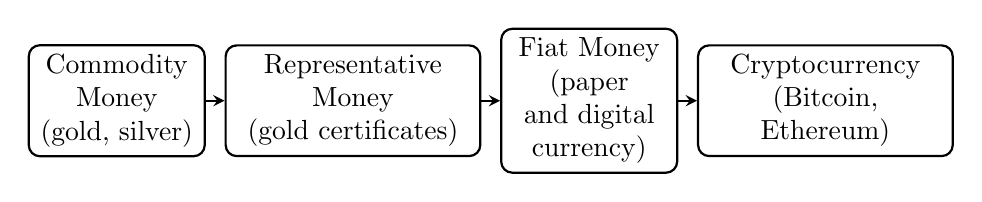
\begin{tikzpicture}[node distance=2.5cm,>=stealth,thick]
      \node (c1) [rectangle, draw, rounded corners, text width=2cm, align=center] {Commodity Money \\ (gold, silver)};
      \node (c2) [rectangle, draw, rounded corners, right of=c1, xshift=0.5cm, text width=3cm, align=center] {Representative Money \\ (gold certificates)};
      \node (c3) [rectangle, draw, rounded corners, right of=c2, xshift=0.5cm, text width=2cm, align=center] {Fiat Money \\ (paper and digital currency)};
      \node (c4) [rectangle, draw, rounded corners, right of=c3, xshift=0.5cm, text width=3cm, align=center] {Cryptocurrency \\ (Bitcoin, Ethereum)};

      \draw[->] (c1) -- (c2);
      \draw[->] (c2) -- (c3);
      \draw[->] (c3) -- (c4);
    \end{tikzpicture}
  \end{center}
  \textit{The evolution of money reflects a shift from tangible, intrinsic value to trust-based and digital systems.}\\
  \vspace{1em}
  \textbf{Contrast:}
  \begin{itemize}
    \item Before 1971, many currencies were \textit{representative money} backed by gold.
    \item Today, all major currencies are purely \textit{fiat}.
  \end{itemize}
\end{frame}

% =========================== Ends Lori Part =========================
% ============================= Begins Yiwen Part ==============================

\section{Model}
\begin{frame}{Model Framework}
  \begin{itemize}
    \item \textbf{Global game approach} to analyze breakdown of trust
    \item Three dates: $[0, 1, 2]$
    \item Continuum $[0,1]$ of risk-neutral merchants, endowed with 1 unit of wealth
    \item Two types of money:
          \begin{itemize}
            \item Bank money (deposits at Bank of Amsterdam)
            \item Metal coins (numeraire, price = 1)
          \end{itemize}
  \end{itemize}
  \begin{block}{Economic Fundamentals}
    $$\theta \sim N(y, 1/\alpha)$$
    \begin{itemize}
      \item $\theta$: True state of economy (trade volume, economic health)
      \item $y$: Public prior mean
            % \item $\alpha$: Precision of public information
    \end{itemize}
  \end{block}
\end{frame}

\begin{frame}{Information Structure: Global Game Approach}
  \begin{itemize}
    \item Each merchant observes private signal:
          \[
            v_i = \theta + \epsilon_i, \quad \epsilon_i \sim N(0, 1/\beta)
          \]
    \item Bank observes $\theta$, merchants only know their $v_i$, $\beta$: Precision of private information
  \end{itemize}
  \begin{block}{Utility from Bank Money}
    \[
      u_i(m) = v_i \cdot f(m)
    \]
    \begin{itemize}
      \item $v_i$: Merchant's private valuation
      \item $f(m)$: \textbf{Network effects} from aggregate adoption
      \item $f(m)$ bounded, increasing, with $f(0) > 0$
    \end{itemize}
  \end{block}
\end{frame}

\begin{frame}{Network Effects}

  \begin{block}{Portfolio Choice}
    Merchant holds bank money if and only if:
    \[
      \mathbb{E} \left[ \frac{v_i \cdot f(m)}{1 + \bar{\gamma}} \right] \geq 1
    \]
    where $\bar{\gamma}$ is the target agio (premium)
  \end{block}

  \begin{alertblock}{Strategic Complementarity}
    The more others use bank money ($m \uparrow$), the more valuable it becomes ($f(m) \uparrow$)
  \end{alertblock}
\end{frame}

\begin{frame}{Bank's Balance Sheet and Policy}
  \begin{columns}
    \begin{column}{0.5\textwidth}
      \begin{block}{Balance Sheet Identity}
        \[
          C + L = M + E
        \]
        \begin{itemize}
          \item $C$: Coins (liquid assets)
          \item $L$: Loans to VOC (illiquid assets)
          \item $M$: Bank money (liabilities)
          \item $E$: Equity (often negative)
        \end{itemize}
      \end{block}
    \end{column}
    \begin{column}{0.5\textwidth}
      \begin{block}{Monetary Policy Operations}
        \begin{itemize}
          \item Target agio $\bar{\gamma} > 0$
          \item Maintain $p = 1 + \bar{\gamma}$
          \item Adjust $M$ via coin sales/purchases
                \begin{itemize}
                  \item Buy coins $\Rightarrow$ Create money $\Rightarrow$ Lower agio
                  \item Sell coins $\Rightarrow$ Destroy money $\Rightarrow$ Raise agio
                \end{itemize}
        \end{itemize}
      \end{block}
    \end{column}
  \end{columns}
\end{frame}

\begin{frame}{The Critical Asymmetry}
  \begin{columns}
    \begin{column}{0.5\textwidth}
      \begin{block}{Easy: Monetary Expansion}
        \begin{itemize}
          \item Can always \textbf{create} money
          \item Buy coins (no upper bound)
          \item Increases $M$, decreases agio
        \end{itemize}
      \end{block}
    \end{column}
    \begin{column}{0.5\textwidth}
      \begin{block}{Hard: Monetary Contraction}
        \begin{itemize}
          \item Limited ability to \textbf{destroy} money
          \item Need coins to sell
          \item Requires $C > 0$
        \end{itemize}
      \end{block}
    \end{column}
  \end{columns}

  \begin{alertblock}{The Binding Constraint}
    When $C = 0$, the bank hits the \textbf{hard limit}:
    \[
      M \geq L - E
    \]
    Cannot reduce money supply below illiquid assets minus equity
  \end{alertblock}
\end{frame}

\begin{frame}{Switching Strategies and Equilibrium}
  \begin{itemize}
    \item Merchants use \textbf{switching strategies}: hold bank money iff $v_i \geq v^*$
          \begin{itemize}
            \item $v^*$: Critical threshold type
            \item Merchants with optimistic signals ($v_i$ high) use bank money
            \item Merchants with pessimistic signals ($v_i$ low) use coins
          \end{itemize}
  \end{itemize}
  \begin{block}{Marginal Type Condition}
    The indifferent merchant ($v_i = v^*$) satisfies:
    \[
      \frac{v^*}{1 + \bar{\gamma}} \cdot F(v^*, y) = 1
    \]
    where $F(v^*, y) = \mathbb{E}[f(m)|v^*, y]$ is expected network benefit
  \end{block}
\end{frame}

\begin{frame}{Characterizing the Equilibrium}
  \begin{block}{Key Lemma}
    CDF of aggregate money holdings:
    \[
      G(m|v^*, y) = \Phi \left( \frac{\alpha}{\sqrt{\alpha + \beta}} (v^* - y) + \sqrt{\frac{\alpha + \beta}{\beta}} \Phi^{-1}(m) \right)
    \]
  \end{block}
  \begin{block}{Money Demand Function}
    Given economic state $\theta$, demand for bank money is:
    \[
      D(\theta) = \Pr(v_i \geq v^*|\theta) = \Phi\left(\sqrt{\beta}(\theta - v^*)\right)
    \]
    \begin{itemize}
      \item Increasing in $\theta$ (better economy $\Rightarrow$ more demand)
      \item Depends on threshold $v^*$
    \end{itemize}
  \end{block}
\end{frame}

\begin{frame}{Break Point}
  \begin{block}{The Critical Moment}
    The \textbf{break point} $\theta^*$ occurs when:
    \begin{enumerate}
      \item Economic fundamentals deteriorate ($\theta$ falls)
      \item Money demand decreases: $D(\theta) \downarrow$
      \item Bank must sell coins to maintain agio
      \item Eventually runs out of coins: $C = 0$
    \end{enumerate}
  \end{block}

  \begin{block}{Mathematical Definition}
    When $C = 0$, from balance sheet identity:
    $M = L - E$

    The break point $\theta^*$ solves:
    \[
      D(\theta^*) = L - E
    \]
    \[
      \Phi\left(\sqrt{\beta}(\theta^* - v^*)\right) = L - E
    \]
  \end{block}
\end{frame}

\begin{frame}{Solving for the Break Point}
  \begin{block}{Closed-Form Solution}
    \[
      \theta^* = v^* + \frac{\Phi^{-1}(L - E)}{\sqrt{\beta}}
    \]
    \begin{itemize}
      \item $\theta^* \uparrow$ as $L \uparrow$ (more illiquid loans)
      \item $\theta^* \uparrow$ as $E \downarrow$ (more negative equity)
      \item $\theta^* \downarrow$ as $\beta \uparrow$ (better information)
    \end{itemize}
  \end{block}

  \begin{alertblock}{Policy Insolvency}
    When $\theta < \theta^*$:
    \begin{itemize}
      \item Bank cannot maintain target agio
      \item Fiat money loses credibility
      \item Coordination on coins instead of bank money
    \end{itemize}
  \end{alertblock}
\end{frame}
% =========================== End Yiwen Part =========================

% =========================== Begins Vivi Part =========================


\begin{frame}{Public perceptions and Weak fundamentals}
  \begin{block}{Step-function}
    \begin{itemize}
      \item Information is private (uncertain): diversity of beliefs smooths out collective response - smooth money demand function
      \item Information is public (common knowledge): $\beta, \alpha \rightarrow \infty$; everyone knows fundamentals are weak -  \textbf{money demand function becomes step function}
      \item The system suddenly flips when $\alpha$ and $\beta$ jointly fall below a critical threshold: A coordination switch driven by shared pessimism about fundamentals
      \item Step function: Either collapse or system is stable, since everyone does the same.
    \end{itemize}
  \end{block}

  \[
    D(\theta) =
    \begin{cases}
      0, & \text{if } \theta < \theta^*,   \\[6pt]
      1, & \text{if } \theta \ge \theta^*.
    \end{cases}
  \]
\end{frame}

\begin{frame}{Break point of economics fundamentals}
  The "break point"' $\theta^*$ is the threshold value of $\theta$ below which trust in bank money collapses.
  \[
    \begin{cases}
      \text{If } \theta \geq \theta^*, & \text{merchants trust and use bank money } \rightarrow \text{ value stays positive}, \\[6pt]
      \text{If } \theta < \theta^*,    & \text{no one wants to hold bank money } \rightarrow \text{ value collapses to zero.}
    \end{cases}
  \]


  \textbf{How does $\theta^*$ move when fundamentals and information change?}\\
  \medskip
  \begin{itemize}
    \item When average fundamentals (mean $y$) fall $\;\Rightarrow\;$ $\theta^*$ rises: It takes less deterioration to reach collapse. The system becomes more fragile.
    \item With public information the bar for maintaining trust gets higher: $\theta^*$ rises.
  \end{itemize}

\end{frame}

% =========================== Ends Vivi Part =========================

% ======================= Begins Lori Part =======================

\section{History of Bank of Amsterdam (1609 \texorpdfstring{$\rightarrow$}{->} 1820)}
\begin{frame}{Chronology at a Glance}
  \begin{center}
    \includegraphics[width=0.87\linewidth]{pasted-images/history.png}
  \end{center}
\end{frame}

\begin{frame}{Single-Name Concentration Risk: VOC (Dutch East India Company)}
  \begin{columns}[T,onlytextwidth]
    \column{0.60\textwidth}
    \begin{center}
      \includegraphics[width=\linewidth]{pasted-images/bank_diagram.png}
    \end{center}
    \vspace{1mm}

    \column{0.40\textwidth}
    \footnotesize
    \vspace{1cm}
    \begin{itemize}
      \item VOC \emph{deposits} at the Bank $\Rightarrow$ the VOC is simultaneously a \emph{major borrower and depositor}.
      \item \emph{Merchants} supply deposits to the Bank and \emph{equity} to the VOC
            % $\Rightarrow$ same agents sit on both sides of the balance-sheet nexus.
    \end{itemize}
  \end{columns}
  \footnotesize
  \begin{itemize}
    \item Two-Sided Exposure \& Feedback Loops:
          \begin{enumerate}
            \item Periodically the Bank has to swap liquid coins $C \downarrow$ for illiquid VOC loans $L \uparrow$
            \item The Bank loses capacity to \emph{contract} money on demand $\Rightarrow$ cannot defend the \textbf{AGIO} $\Rightarrow$ \textbf{policy insolvency}
          \end{enumerate}
    \item \emph{Wrong-way risk}: when the VOC weakens, its \emph{loan quality falls} while its \emph{deposits shrink}.
  \end{itemize}
\end{frame}

\begin{frame}{Anglo-Dutch War (1780-1784) \texorpdfstring{$\rightarrow$}{->} Risk Materializes}
  \begin{itemize}
    \item \textbf{War shock:} Fourth Anglo-Dutch War (1780-1784) severely impairs VOC trade:
          \begin{itemize}
            \item VOC \textbf{sales collapse}: From \textasciitilde{}21m $\rightarrow$ To <6m guilders in \textbf{1780-1781}.
          \end{itemize}
    \item \textbf{Policy error:} Bank \textbf{doubles down} on VOC credit risk instead of de-risking.
          \begin{itemize}
            \item \textbf{VOC loans peak (1783):} \textbf{7.8m} guilders $\approx$ \textbf{71\%} of total bank assets (extreme concentration \& illiquidity).
          \end{itemize}
  \end{itemize}
  \begin{center}
    \includegraphics[width=0.8\linewidth]{pasted-images/voc_sales.png}
  \end{center}
\end{frame}

\begin{frame}{Balance-Sheet Deterioration \& Loss of Backing}
  \textbf{Policy error:} Bank \textbf{doubles down} on VOC credit risk instead of de-risking.
  \begin{itemize}
    \item \textbf{VOC loans peak (1783)} $\Rightarrow$ extreme concentration \& illiquidity (\textbf{7.8m} guilders $\approx$ \textbf{71\%} of total bank assets)
    \item \textbf{Liquid reserves drain:} Metals drop from \textbf{\textasciitilde{}17m (1776)} $\rightarrow$ to \textbf{\textasciitilde{}7.8m (1783)}.
    \item \textbf{Backing ratio:} \textbf{\textasciitilde{}97\% (1776)} $\rightarrow$ \textbf{\textasciitilde{}28\% (1783)} of bank guilders backed by metal.
    \item \textbf{Missing fiscal backstop:} City of Amsterdam lacked sovereign-scale capacity to \textbf{recapitalize} credibly.
  \end{itemize}
  \begin{center}
    \includegraphics[width=0.8\linewidth]{pasted-images/encumbered_accounts.png}
  \end{center}
\end{frame}

\begin{frame}{Market Signals \& Timeline of Confidence Erosion}
  \begin{itemize}
    \item \textbf{AGIO slippage:}
          \begin{itemize}
            \item \textbf{July 1789:} AGIO $\approx$ \textbf{2\%} (below target band).
            \item \textbf{Oct 1790-Feb 1791:} \textbf{AGIO turns negative} (inferior to ``dodgy'' coins).
          \end{itemize}
    \item \textbf{Transparency shock (1795):} French invasion $\rightarrow$ Batavian Republic opens the books; insolvency revealed.
          \begin{itemize}
            \item Public information revelation $\rightarrow$ \textbf{panic}; AGIO \textbf{collapses further} (network effects flip).
          \end{itemize}
  \end{itemize}
  \begin{center}
    \includegraphics[width=0.8\linewidth]{pasted-images/agio_over_time.png}
  \end{center}
\end{frame}

% =========================== Ends Lori Part =========================

\section{Modern Implications}

\begin{frame}{Comparison to Contemporary Central Banking}
  \scriptsize % or \footnotesize
  \centering
  \begin{tabular}{p{2.2cm} p{4.2cm} p{4.2cm}}
    \hline
    \textbf{Concept}  & \textbf{Bank of Amsterdam}                          & \textbf{Modern Central Banks}                                      \\
    \hline
    Issuer            & Municipal bank with no fiscal backstop              & Central banks with national governments                            \\
    Users             & Merchants holding ``bank money''                    & Commercial banks holding reserves                                  \\
    Value anchor      & Agio vs.\ coins (metal money)                       & Exchange rate vs.\ other currencies                                \\
    Crisis trigger    & Negative equity + illiquid assets + lost confidence & Same combination — worsened by high rates and weak fiscal capacity \\
    Stabilizing force & None (no fiscal support)                            & Government recapitalization and credibility
  \end{tabular}
\end{frame}

\begin{frame}{Core Idea: Trust Break Point in Fiat Regimes}
  \begin{itemize}
    \item Model insight: there exists a \emph{unique break point} where trust in fiat money collapses when shocks are severe, bank equity turns deeply negative, and fiscal support is lacking.
    \item Network effects can sustain fiat systems for a while, but without credible backstops solvency concerns can flip expectations quickly (step-like collapse).
    \item Comparison to today: modern central banks rely on credibility and fiscal backing to keep the ``agio'' (exchange value of money) anchored despite losses.
  \end{itemize}
\end{frame}

\begin{frame}{Importance of Fiscal Backstop}
  \begin{figure}
    \centering
    \includegraphics[width=\textwidth, height=0.75\textheight, keepaspectratio]{pasted-images/Scenario war.png}
    \label{fig:placeholder}
  \end{figure}

  \scriptsize
  With Fiscal Backing:
  \begin{itemize}
    \item Inject capital (recapitalization)
    \item Guarantee its liabilities (legal tender laws, deposit insurance)
    \item Issue government bonds to replenish reserves
  \end{itemize}
\end{frame}



\begin{frame}{Policy Takeaways for Today}
  \begin{itemize}
    \item Preserve \textbf{sound central-bank finances} ex ante (risk management, capital buffers) to avoid approaching the break point.
    \item Ensure \textbf{credible, transparent fiscal backstops}; design legal frameworks for swift recapitalisation in stress.
    \item Recognise that \textbf{equity shortfalls} can be tolerated temporarily, but not if they coincide with severe shocks \emph{and} absent fiscal support.
    \item Communication: emphasise the state-contingent path where monetary and fiscal authorities act jointly to defend the value of money.
  \end{itemize}
\end{frame}


\section{Conclusion}

\begin{frame}{Summary of Contributions}
  \begin{block}{Theoretical Innovation}
    \begin{itemize}
      \item Global game model of fiat money collapse
      \item Microfoundations for network effects in money demand
      \item Unique characterization of break point
      \item Role of public information in coordination failure
    \end{itemize}
  \end{block}

  \begin{block}{Policy Considerations}
    \begin{itemize}
      \item Framework for analyzing modern central bank risks
      \item Balance sheet constraints matter
      \item Sound central bank finances and fiscal backing are essential public goods
    \end{itemize}
  \end{block}
\end{frame}

\section{Appendix}

\begin{frame}{The economic roles of $\alpha$ and $\beta$}
  \begin{block}{Theoretical Innovation}
    \begin{itemize}
      \item Global game model of fiat money collapse
      \item Microfoundations for network effects in money demand
      \item Unique characterization of break point
      \item Role of public information in coordination failure
    \end{itemize}
  \end{block}

  \begin{block}{Policy Considerations}
    \begin{itemize}
      \item Framework for analyzing modern central bank risks
      \item Balance sheet constraints matter
      \item Sound central bank finances and fiscal backing are essential public goods
    \end{itemize}
  \end{block}
\end{frame}


\begin{frame}{Related Literature \& This Paper’s Novelty}
  \footnotesize
  \textbf{1) Diamond \& Dybvig (1983) — deposit runs, liquidity mismatch}
  \begin{itemize}
    \item Classic bank-run framework (private bank default under liquidity shock).
    \item \textit{Novel Contribution:} Not a run model; Focus is on \textbf{money demand with network effects} and the capacity to contract $M$ to defend a target relative price.
  \end{itemize}

  \textbf{2) Krugman (1979); Morris \& Shin (1998, 2003) — currency crises \& global games}
  \begin{itemize}
    \item Peg attacks and unique-equilibrium selection via global games (speculators vs.\ peg credibility).
    \item \textit{Novel Contribution:} Global game in \textbf{private values over money demand}, with a \textbf{balance-sheet constraint} pinning a \emph{unique break point}: when $C\!\to\!0$, market clearing requires $M \ge L-E$; below a fundamentals threshold $v^*$, agio cannot be held. As public information improves, outcomes approach a \textbf{step function} (discrete trust collapse).
  \end{itemize}

  \textbf{3) Schilling, Fernández\textendash Villaverde \& Uhlig (2020) — CBDC runs/trade-offs}
  \begin{itemize}
    \item CB can always print to meet CBDC obligations but may sacrifice the inflation target; no alternative means of payment in the setup.
    \item \textit{Novel Contribution:} \textbf{Alternatives exist} (coins/other monies), and the issuer must sometimes \textbf{shrink money} (QT) to defend the agio; introduces a \textbf{hard liquid-asset constraint} (need sellable $C$) and highlights the role of a \textbf{credible fiscal backstop} for policy solvency.
  \end{itemize}

\end{frame}

\begin{frame}
  \centering
  \Large
  Thank you!\\
  Questions?
\end{frame}


\end{document}